\documentclass[12pt, twoside, final, openany]{mgr}
\usepackage{indentfirst}
\usepackage[T1]{fontenc}
\usepackage{polski}      
\usepackage[UTF8]{inputenc}
\usepackage{lmodern}
\usepackage[nolabel]{showlabels}


%pakiety do grafiki
\usepackage{graphicx}
\usepackage{subfigure}
\usepackage{psfrag}

%pakiety dodające dużo dodatkowych poleceń matematycznych
\usepackage{amsmath}
\usepackage{amsfonts}

%pakiety wspomagające i poprawiające składanie tabel
\usepackage{supertabular}
\usepackage{array}
\usepackage{tabularx}
\usepackage{hhline}

%pakiet wypisujący na marginesie etykiety równań i rysunków
%zdefiniowanych przez \label{}, chcąc wygenerować finalną wersję
%dokumentu wystarczy usunąć poniższą linię
\usepackage{showlabels}

%definicje własnych poleceń
\newcommand{\R}{I\!\!R} %symbol liczb rzeczywistych, działa tylko w
                        %trybie matematycznym
\renewcommand*\descriptionlabel[1]{\hspace\leftmargin$#1$}

\newtheorem{theorem}{Twierdzenie}[section] %nowe otoczenie do
                                           %składania twierdzeń

%dane do złożenia strony tytułowej
\title{Analiza łańcucha transakcji w sieci Bitcoin}
\engtitle{The analysis of Bitcoin transactions blockchain}
\author{Bartosz Zychal}
\supervisor{dr inż. Radosław Michaliski} %\Prof. PWr, I-6
%\guardian{dr hab. inż. Imię Nazwisko Prof. PWr, I-6} %nie używać
%jeśli opiekun jest tą samą osobą co prowadzący pracę

\date{2018} %standardowo u dołu strony tytułowej umieszczany jest
%bieżący rok, to polecenie pozwala wstawić dowolny rok

%poniżej jest lista kierunków i specjalności na wydziale elektroniki,
%należy wybrać właściwe lub dopisać jeśli nie ma odpowiednich
\field{Informatyka (INF)}
\specialisation{Systemy Baz Danych (SBD)}

%tutaj zaczyna się właściwa treść dokumentu
\begin{document}
\def\listtablename{Spis tabel}
\def\tablename{Tabela. }

\maketitle %polecenie generujące stronę tytułową 

\tableofcontents{2} %spis treści
\chapter*{Wprowadzenie}
Do napisania na końcu. Ma zawierać informacje o motywacji i celu pracy. 

\chapter{Kryptowaluty - wprowadzenie}

\section{Krótka definicja} \label{sec:definicjaKryptowaluty}
\indent Krypotowaluta to cyfrowy zasób mogący odpowiadać pewnej wartości środków finansowych. Zasób ten został zaprojektowany w sposób pozwalający określać go jako medium wymiany przy użyciu kryptografii, z którą jest ściśle powiązany. Kryptografia pozwala na zabezpieczenie transakcji, kontrolowanie tworzenia nowych jednostek kryptowaluty oraz weryfikację ilości posiadanych jej jednostek. Aktualnie krypotwaluty klasyfikowane są do trzech grup:
\begin{itemize}
\item walut cyfrowych
\item walut alternatywnych
\item walut wirtualnych
\end{itemize}

\section{Bezpieczeństwo w walutach i kryptowalutach} \label{sec:bezpieczenstwoWwalutach}
\indent Wszystkie waluty muszą być w jakiś sposób kontrolowane i podlegać różnego rodzaju zabezpieczeniom, tak aby zapobiegać oszustwom. W przypadku walut fiducjarnych, tj. walut nie mających pokrycia w dobrach materialnych, organizacje takie jak banki kontrolują podaż pieniądza oraz oznaczają fizycznie walutę, w celu uniemożliwienia jej podrobienia. Takie zabezpieczenia w pewnym stopniu ograniczają możliwości fałszerstwa, jednakże nie dają stuprocentowej pewności. Kryptowaluty podobnie jak tradycyjne waluty muszą posiadać miary zabezpieczeń w celu uniemożliwienia wpływania na stan systemu i tworzenia niekonsystentnych danych. Dodatkowo muszą one posiadać zabezpieczenia niepozwalające na wielokrotne użycie tych samych środków. W przeciwieństwie do walut fiducjarnych zasady bezpieczeństwa kryptowalut mogą bazować wyłącznie na istniejących  technologiach i nie mogą podlegać kontroli ze strony jakiejkolwiek centralnej instytucji. 

\section{Kryptografia} \label{sec:kryptografia}
\indent Kryptowaluty bardzo silnie bazują na kryptografii, która oferuje mechanizm bezpiecznego kodowania zasad ich systemu. Kryptografia pozwala nie tylko bronić system przed manipulacjami i matactwami, ale równie dobrze może zostać użyta w celu kodowania zasad tworzenia nowych jednostek kryptowaluty przy pomocy określonego matematycznego protokołu. 

\indent Kryptografię można sklasyfikować jako dziedzinę wiedzy o zabezpieczeniach przed nieautoryzowanym dostępem do informacji. W dzisiejszych czasach uważa się ją nie tylko za gałąź matematyki, ale i informatyki. Kryptografię można podzielić na:
\begin{itemize}
\item symetrczyną - polega na możliwości odczytania wiadomości przy pomocy tego samego klucza, którą została podpisana. Znaczącym problemem bezpieczeństwa w tym podejściu jest przekazanie odbiorcy klucza. 
\item niesymetrczyną - polega na istnieniu co najmniej dwóch kluczy:
\begin{itemize}
\item prywatny - nazwa klucza pochodzi od faktu, iż klucz ten nie powinien być nigdy nikomu udostępniony. Przy pomocy klucza prywatnego można odszyfrować wiadomość podpisaną kluczem publicznym. Pozwala również na podpisanie wiadomości, która może być później zweryfikowana za pomocą klucza publicznego.
\item publiczny - nazwa klucza pochodzi od faktu, iż klucz ten może zostać bez żadnych zastrzeżeń upubliczniony. Klucz publiczny tworzy się na podstawie klucza prywatnego, jednakże odtworzenie klucza prywatnego z klucza publicznego jest bardzo trudne. Klucz publiczny używany jest do szyfrowania wiadomości oraz weryfikacji wiadomości podpisanej kluczem prywatnym.
\end{itemize}
\end{itemize} 

\indent Kryptografia oparta na kluczu publicznym została opracowana w latach 70. XX wieku i cały czas stanowi solidną podstawę bezpieczeństwa komputerowego i informacyjnego. Od czasu jej powstania odkryto matematyczne funkcje, które są praktycznie nieodwracalne, np. \textit{potęgowanie liczby pierwszej} i \textit{mnożenie krzywych eliptycznych}. Oznacza to że łatwo obliczyć je w jednym kierunku, jednakże operacja odwrotna jest praktycznie niewykonywalna. Bitcoin korzysta z mnożenia krzywej eliptycznej jako podstawy przy wyliczaniu klucza publicznego. Sposób użycia tej funkcji został przedstawiony w podrozdziale ~\ref{sec:tworzenieKluczyPublicznych}.

\section{Zastosowanie kryptografii w sieci Bitcoin} \label{sec:zastosowanieKryptografii}
\indent Aktualnie na rynku dostępne jest ponad tysiąc różnych kryptowalut, a wraz z rosnącym zainteresowaniem oraz zaufaniem społecznym ilość walut cyfrowych cały czas rośnie. Niepodważalny jest fakt, że jedną z najbardziej powszechnych i popularnych kryptowalut jest Bitcoin. Bitcoin jest całkowicie zdecentralizowaną zdigitalizowaną walutą bez globalnego emitenta, który miałby nią zarządzać oraz ją rozpowszechniać. Bazując na specjalistycznym otwartym oprogramowaniu pewna ilość Bitcoinów przekazywana jest użytkownikom w zamian za działania pozwalające na działanie systemu Bitcoin. Użytkownicy Ci zwani są kopaczami, a operacje przez nich wykonywane, w celu podtrzymania systemu zwane są kopaniem. Kopanie Bitcoinów poza zyskiem ze strony kopaczy, daje olbrzymi zysk dla systemu, pozwalając weryfikować zlecone transakcje.

\indent Właściciele Bitcoinów ustalani są na podstawie kluczy cyfrowych, adresów Bitcoin oraz podpisów cyfrowych. Klucze cyfrowe nie są przechowywane w sieci, jednakże są tworzone przez użytkowników oraz przetrzymywane w ich portfelach w plikach lub bazie danych. Klucz cyfrowy jest całkowicie niezależny od protokołu sieci Bitcoin, dlatego też może być tworzony przez różnie oprogramowania. Oprogramowanie to musi zapewniać użycie bezpiecznego źródła entropii w celu wygenerowania unikalnego klucza. Wygenerowanie istniejącego lub zbyt słabego klucza może spowodować, iż w przyszłości użytkownik utraci zebrane środki. Klucze zapewniają w sieci Bitcoin:
\begin{itemize}
\item zdecentralizowane zaufanie
\item zaświadczenie o własności
\item odporny na kryptografię model bezpieczeństwa
\end{itemize}
Transakcje w sieci Bitcoin wymagają dodania prawidłowego podpisu do łańcucha bloków, co dokładniej opisane zostało w rozdziale ~\ref{blockchain}. Podpis ten może być wygenerowany przy pomocy ważnych kluczy cyfrowych. Każdy kto posiada kopię tych kluczy może kontrolować środki dostępne na koncie. Protokół sieci Bitcoin korzysta z szyfrowania asymetrycznego, a co za tym idzie w transakcji klucz publiczny odbiorcy jest prezentowy przez jego odcisk palca, zwany adresem Bitcoin. Adresy te są ogólnodostępne i widoczne przez wszystkich. 

\indent Z klucza publicznego korzysta się w celu odebrania Bitcoinów, natomiast klucz prywatny wymagany jest do wydawania Bitcoinów. Osoba wydająca Bitcoiny musi zaprezentować swój klucz publiczny oraz podpis w transakcji. Podpis za każdym razem jest inny, lecz tworzony z jednego klucza prywatnego, co pozwala na udaną weryfikację przy pomocy dołączonego klucza publicznego. Poprzez załączenie obu tych informacji każdy w sieci może zweryfikować oraz oraz zaakceptować transakcję jako poprawną lub ją odrzucić, w przypadku stwierdzenia, braku środków na adresie nadawcy. 

\indent Klucz prywatny w sieci Bitcoin powiązany jest ścisłe z adresem, dlatego też jego utrata powoduje nieodwracalną utratę środków. Pomimo iż są one cały czas dostępne nie mogą zostać użyte bez prawidłowego podpisu generowanego z klucza prywatnego.

\section{Metoda tworzenia kluczy publicznych na przykładzie sieci Bitcoin} \label{sec:tworzenieKluczyPublicznych}
\indent Jak już wcześniej wspomniano klucz publiczny obliczany jest z klucza prywatnego przy pomocy  \textit{mnożenia krzywej eliptycznej}, Jest on praktycznie nieodwracalny i można go zapisać jako:
\begin{equation}  
\label{eq:1}
  K = k*G, 
\end{equation} 
gdzie:
\begin{description}
\item[k] jest wartością klucza prywatnego,
\item[G] jest stałym punktem zwanym punktem generującym,
\item[K] jest wynikowym kluczem publicznym.
\end{description}

Kryptografia krzywej eliptycznej jest rodzajem kryptografi asymetrycznej bazującej na problemie logarytmu dyskretnego wyrażona jako sumy i iloczyny punktów na tej krzywej eliptycznej. Dlatego też, operacją odwrotną do mnożenia krzywej eliptycznej jest \textit{odnalezienie logarytmu dyskretnego} i wymaga zastosowania wyszukiwania przy pomocy algorytmu typu \textit{brute-force}, czyli przeglądu zupełnego.  

\indent W przypadku Bitcoina parametry krzywej eliptycznej są ściśle określone i zdefiniowane są przy pomocy standardu zwanego \textit{secp256k1}. Standard ten został ustalony przez amerykańską Narodową Instytucję Standaryzacji i Technologii. Zastosowana w tej kryptowalucie  krzywa eliptyczna tworzona jest na podstawie określonego zbioru stałych matematycznych i jest wyrażana przy pomocy funkcji:
\begin{equation}
  y^2 = x^3 + 7 
\end{equation} 
\label{eq:2}
lub:
\begin{equation} 
\label{eq:3}
  y2 \mod p = (x^3 + 7) \mod p
\end{equation}
Moduł liczby pierwszej \textit{mod p} implikuje właściwość krzywej jako znajdującej się nad skończonym polem pierwszego rzędu p. Można ją również zapisać jako funkcję $F_p$, gdzie $p = 2^{256} - 2^{32} - 2^9 - 2^8 - 2^7 - 2^6 - 2^4 - 1$ jest olbrzymią liczbą pierwszą. Oznacza to, iż od pewnego momentu krzywa zdefiniowana jest przy pomocy liczb zespolonych, a nie rzeczywistych. Utrudnia to jej wizualizację, gdyż wykres takiej funkcji musiałby zostać przedstawiony w dwóch wymiarach i składał by się z wielu pojedynczych punktów w przestrzeni. Na potrzeby graficznego przedstawienia  uproszczono wykres \ref{fig:krzywaEliptyczna} funkcji ~\ref{eq:2} przedstawiając go tylko w świecie liczb rzeczywistych. Wykres ten został podzielony na dwa obszary przy pomocy pionowej kreski, która nie jest częścią wykresu funkcji. Lewy obszar obejmuje wartości funkcji w świecie liczb zespolonych, który pominięto, natomiast prawa strona wykresu przedstawia funkcję \ref{eq:2}, w świecie liczb rzeczywistych. 
\begin{figure}[h]
\centering
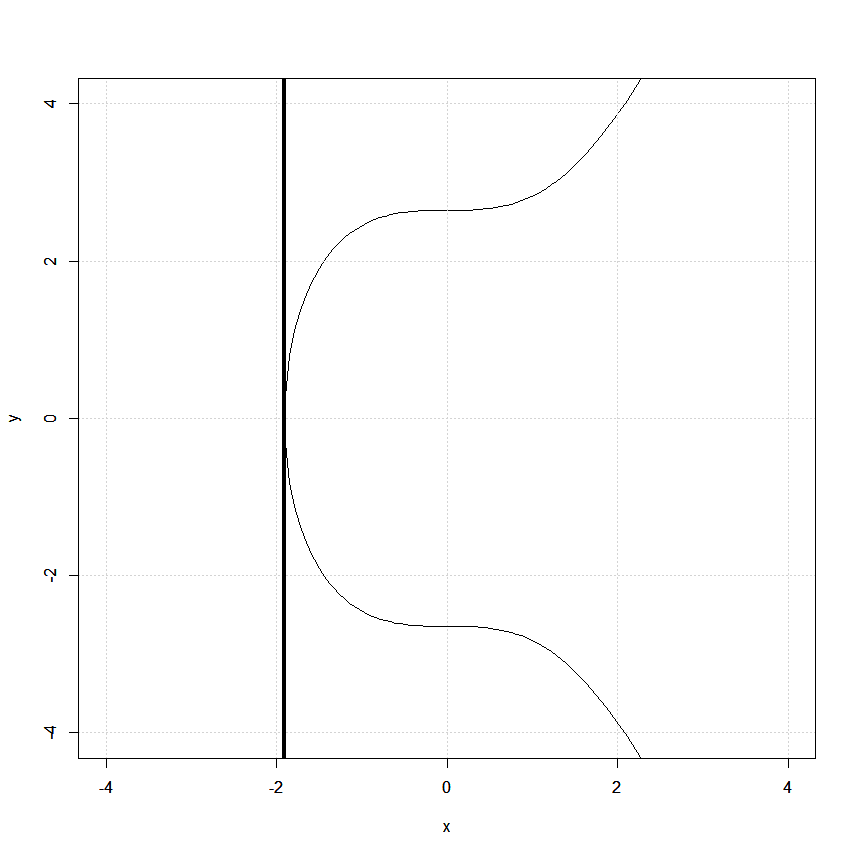
\includegraphics[width=0.9\linewidth]{pictures/elliptic.png}
\caption{Krzywa eliptyczna zastosowana do wyznaczenia wartości G w protokole Bitcoin}
\label{fig:krzywaEliptyczna}
\end{figure}

Parametr \textit{G} został wybrany na podstawie powyższej krzywej eliptycznej przez protokół Bitcoina przy użyciu standardu \textit{secp256k1}. Parametr ten jest przypisywany do wszystkich użytkowników sieci. Implikuje to wygenerowanie za każdym razem takiego samego klucz publicznego na podstawie tego samego klucza prywatnego. Klucz prywatny może mieć wartość od $1$ do prawie $2^{256}$, a zależność pomiędzy jego wartością \textit{k} i wartością klucza publicznego \textit{K} jest stała. Oznacza to, że aby przy znajomości stałej wartości \textit{G} odtworzyć wartość klucza publicznego \textit{k} wymagany jest przegląd wszystkich możliwych wartości klucza prywatnego \textit{k}. 

\section{Podsumowanie} \label{sec:podsumowanieKryptowaluty}
\indent Reasumując za każdą walutą musi stać jakiś określony system zabezpieczeń. W przypadku tradycyjnych walut są to centralne instytucje nadzorujące obrót i podaż określonego pieniądza. W przypadku kryptowalut bezpieczeństwo zapewnione jest poprzez zastosowanie prostej w użyciu, aczkolwiek skomplikowanej w budowie kryptografii. Zapewnia to możliwości bardzo szybkiej weryfikacji posiadanych środków, przy bardzo niskim nakładzie pracy. Dodatkowo kryptografia w porównaniu do tradycyjnych metod zabezpieczania pieniądza, nie pozwala na kontrolowanie przez jedną osobę, organizację czy instytucję poprawności danych. To zadanie wykonywane jest przez wszystkich kopaczy w sieci Bitcoin. 


\chapter{Blockchain - rejest transakcji}
\label{blockchain}

\chapter{Przegląd metod analiz sieci złożonych (też temporalnych) oraz analiz blockchaina}

\chapter{Część eksperymentalna}
\section{Plan badań}
\section{Analiza blockchaina Bitcoin}
\section{Wnioski}


\chapter*{Podsumowanie}


\addcontentsline{toc}{chapter}{Bibliografia} %utworzenie w
                                             %spisietreści pozycji
                                             %Bibliografia

\bibliography{bibliografia} % wstawia bibliografię korzystajšc z pliku
                            % bibliografia.bib - dotyczy BibTeXa,
                            % jeżeli nie korzystamy z BibTeXa należy
                            % użyć otoczenia thebibliography

%opcjonalnie może się tu pojawić spis rysunków i tabel
% \listoffigures
% \listoftables
\end{document}

